\documentclass[tikz, convert={density=300,size=1920x1080,outext=.png}]{standalone}

\usepackage{xcolor}

\newcommand{\len}{10}
\newcommand{\bre}{10}
\newcommand{\hei}{5}
\newcommand{\frontcolor}{black!15!white}
\newcommand{\topcolor}{black!30!white}
\newcommand{\sidecolor}{black!45!white}

\begin{document}
    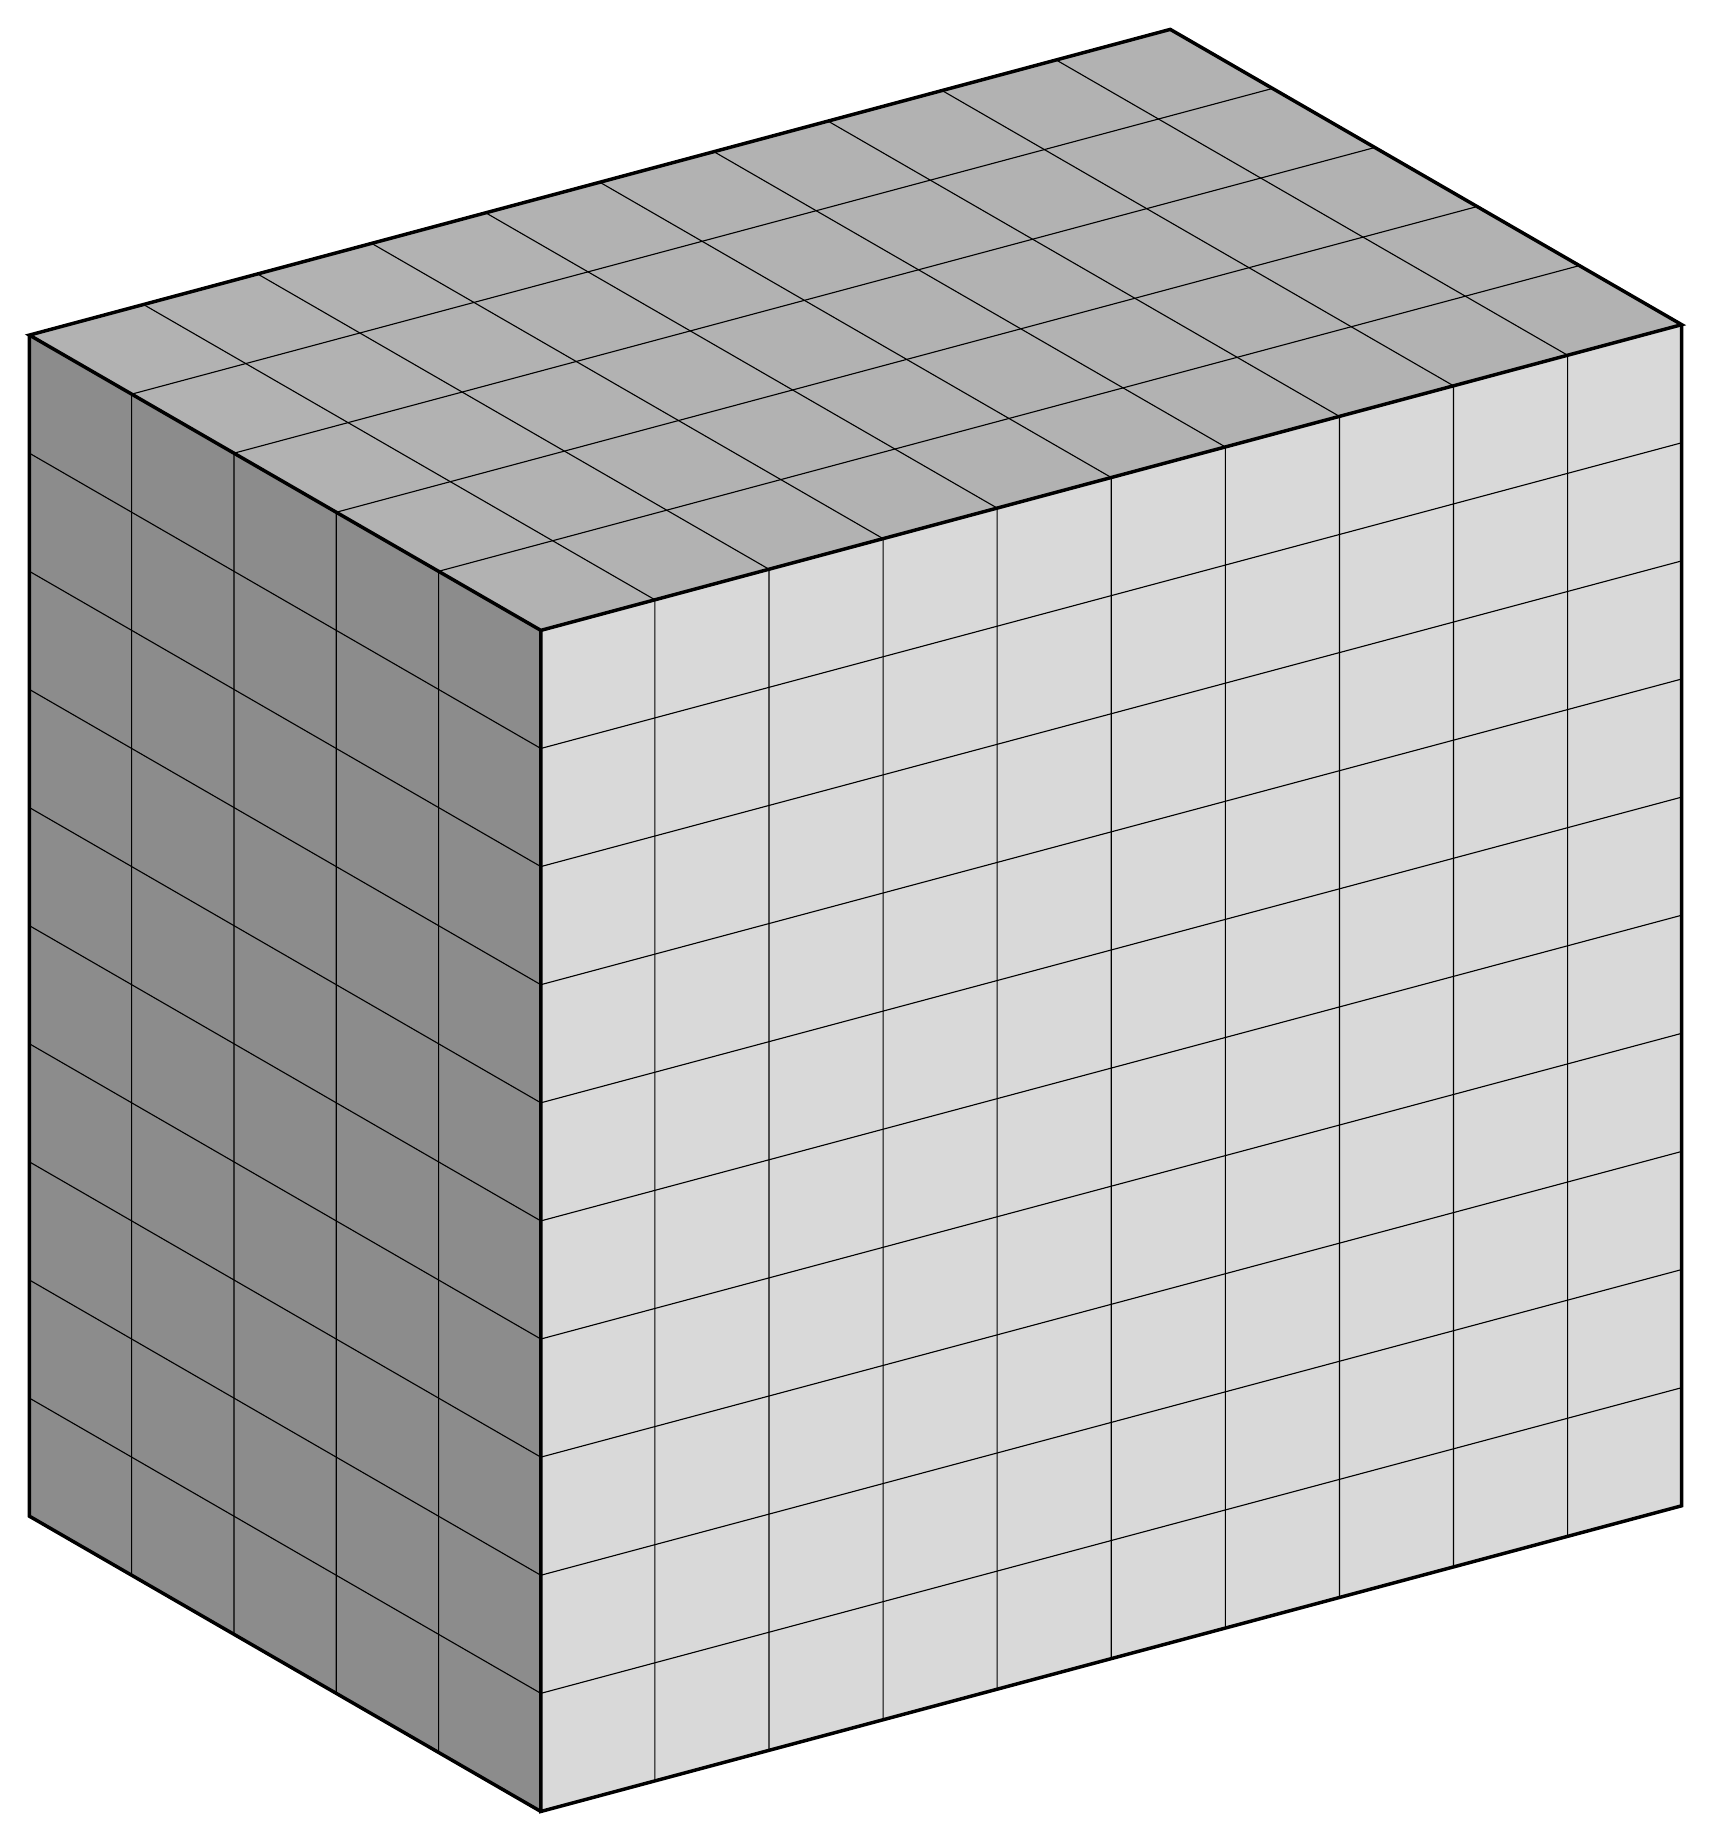
\begin{tikzpicture}[x=(15:1.5cm), y=(90:1.5cm), z=(330:1.5cm), >=stealth]
        \coordinate (O) at (0, 0, 0);
        \coordinate (A) at (\len, 0, 0);
        \coordinate (B) at (0, \bre, 0);
        \coordinate (C) at (\len, \bre, 0);
        \coordinate (D) at (0, 0, \hei);
        \coordinate (E) at (\len, 0, \hei);
        \coordinate (F) at (0, \bre, \hei);
        \coordinate (G) at (\len, \bre, \hei);
        
        \fill[\frontcolor] (D) -- (E) -- (G) -- (F) -- cycle;
        \fill[\topcolor] (B) -- (C) -- (G) -- (F) -- cycle;
        \fill[\sidecolor] (O) -- (B) -- (F) -- (D) -- cycle;
        % draw dotted dividing lines
        \foreach \z in {1, ..., 4}
            \draw[-] (0, 0, \z) -- (0, \bre, \z) -- (\len, \bre, \z); 
        \foreach \x in {1, ..., 9}
            \draw[-] (\x, 0, \hei) -- (\x, \bre, \hei) -- (\x, \bre, 0);
        \foreach \y in {1, ..., 9}
            \draw[-] (0, \y, 0) -- (0, \y, \hei) -- (\len, \y, \hei);
        \draw[line width=1.25pt] (B) -- (F) -- (G) -- (C) -- cycle;
        \draw[line width=1.25pt] (F) -- (D) -- (E) -- (G);
        \draw[line width=1.25pt] (B) -- (O) -- (D);
        
        
%        \draw[thick, gray] (10, 0, 0) -- (10, -10, 0) -- (0, -10, 0);
%        \draw[thick, gray] (10, -10, 0) -- (10, -10, 5);
%        % draw dotted dividing lines
%        \foreach \z in {1, 2, 3, 4}
%            \draw[dashed] (10, 0, \z) -- (0, 0, \z) -- (0, -10, \z); 
%        \foreach \x in {1, ..., 9}
%            \draw[dashed] (\x, 0, 0) -- (\x, 0, 5) -- (\x, -10, 5);
%        \foreach \y in {-9, ..., -1}
%            \draw[dashed] (0, \y, 0) -- (0, \y, 5) -- (10, \y, 5);
%        \draw[thick] (0, 0, 0) -- (10, 0, 0) -- (10, 0, 5) -- (0, 0, 5) -- cycle;
%        \draw[thick] (0, 0, 0) -- (0, -10, 0) -- (0, -10, 5) -- (0, 0, 5);
%        \draw[thick] (0, -10, 5) -- (10, -10, 5) -- (10, 0, 5);
        
        
    \end{tikzpicture}
\end{document}